%||||---------------
\begin{frame}[ctb!]
  \frametitle{NESD's Role: In General}
  Every year NESD meets for around 4 days.
  \begin{itemize}
    \item Meet with administration and others
      \begin{itemize}
        \item DOE - Assistant Secretary Lyons
        \item NRC - Commissioner Magwood
        \item CBO
        \item NEI
      \end{itemize}
    \item Write a policy statement
    \item Meet with representatives
  \end{itemize}
\end{frame}
%---------------||||

%||||---------------
\begin{frame}[ctb!]
  \frametitle{NESD's Role: A Student Voice}
  We try to provide the student's perspective to law makers via
  a policy statement.
  \begin{figure}[htbp!]
    \begin{center}
      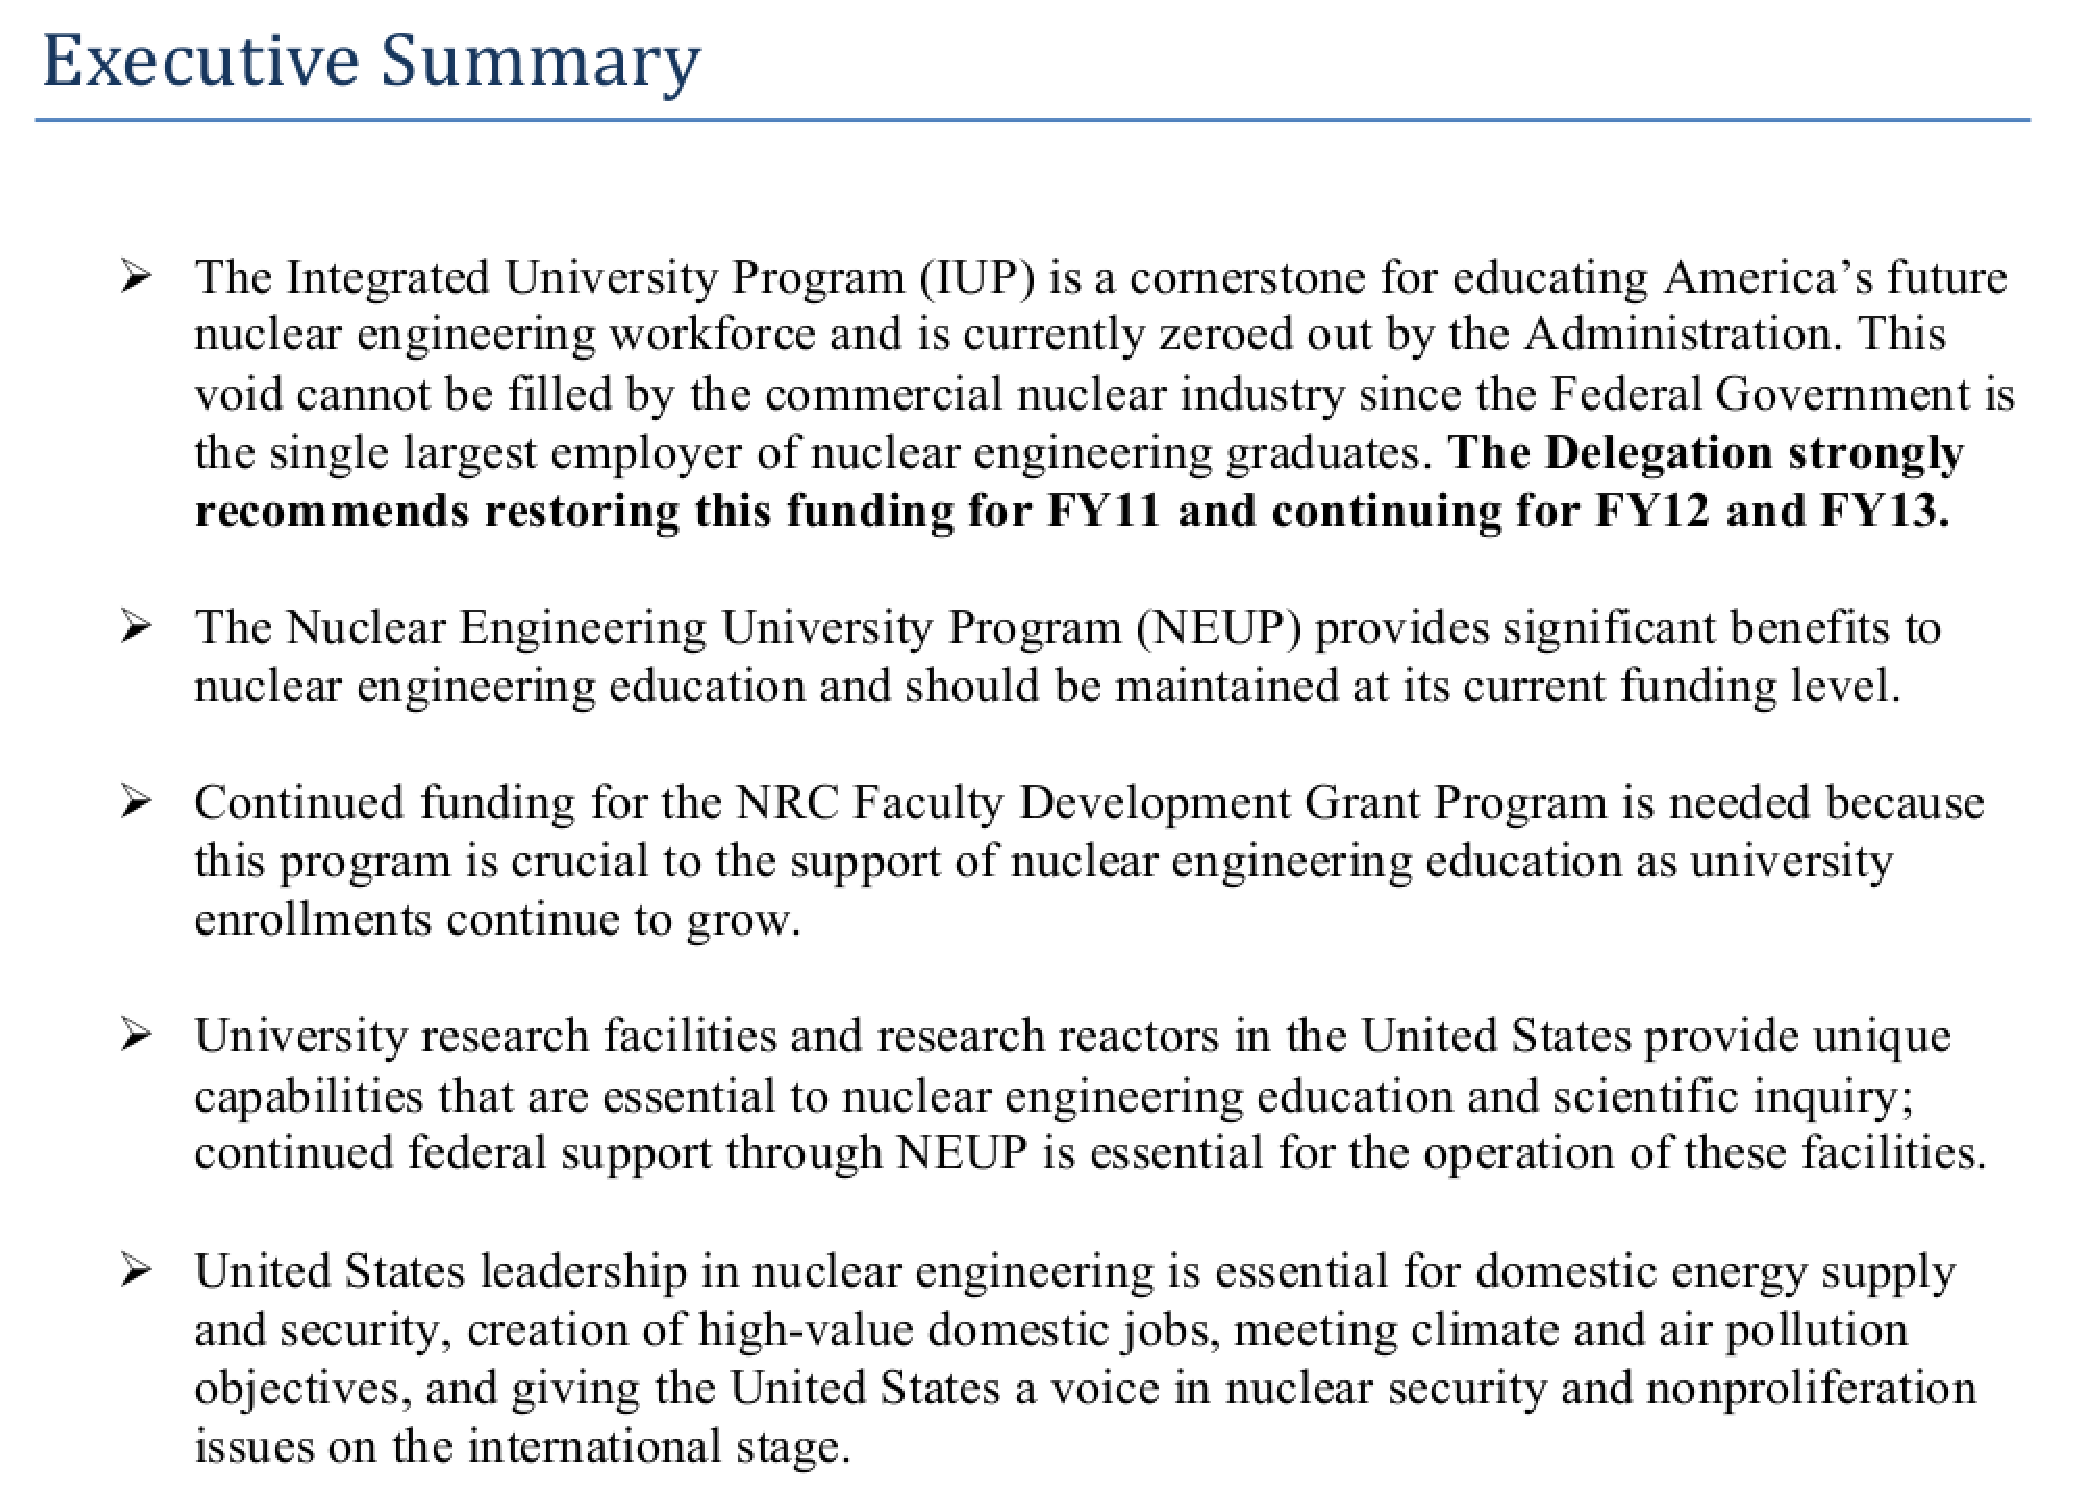
\includegraphics[height=5.5cm]{exec.eps}
    \caption{NESD 2011 Executive Summary}
    \label{fig:exec}
    \end{center}
  \end{figure}
\end{frame}
%---------------||||

%||||---------------
\begin{frame}[ctb!]
  \frametitle{NESD's Role: This Year}
  We will again enter a climate where the administration has
  zeroed out much of IUP.
  \vspace{0.4cm}
  \pause
  
  From ANS President, Eric Loewen's testimony\cite{loewen_testimony_2012}:
  \begin{quote}
    We urge the Subcommittee to support the continuation of the 
    Integrated University Program. Specifically, we request that 
    the Subcommittee to restore the full \$15 million in funding 
    for the Nuclear Regulatory Commission's portion of the IUP
    program and the \$5 million FY12 appropriated level for DOE-NE. 
  \end{quote}
\end{frame}
%---------------||||
